\documentclass[11pt]{article}

\usepackage[english]{babel}
\usepackage[usenames,dvipsnames,svgnames,table]{xcolor}
\usepackage{mdframed,graphics}
\usepackage{amsmath,amssymb,epsfig,graphics,hyperref,amsthm,placeins,mathtools}

\definecolor{light-gray}{gray}{0.8}

\setlength{\textwidth}{7in}
\setlength{\topmargin}{-0.575in}
\setlength{\textheight}{9.25in}
\setlength{\oddsidemargin}{-.25in}
\setlength{\evensidemargin}{-.25in}

\title{Protocols Performance Comparison}
\author{Shuo Yang}

\begin{document}
\maketitle

\section*{Intro}
I used two programs to compare the performance between mirror and
parallel protocols. The first one is red-black grid computing from
our programming project 1. The other one is a test case written by
myself. Both programs ran on 8 nodes (4 primary nodes and 4 replicas) on
the 9th floor. I will show the results of both and briefly explain the
reasons. 

\section*{Red-black Test}
Red-black test ran on a grid of size 8080 for 30 iterations. It
contains 4 sub-tests: 1) \emph{all nodes are alive} during the
execution; 2) \emph{2 primary nodes were killed} in the mid of the
execution; 3) \emph{2 replica nodes were killed} in the mid of the
execution; 4) \emph{a primary node and a replica node were killed} in
the mid of the execution. The results are shown in the Figure 1.

\begin{figure}
  \centering
  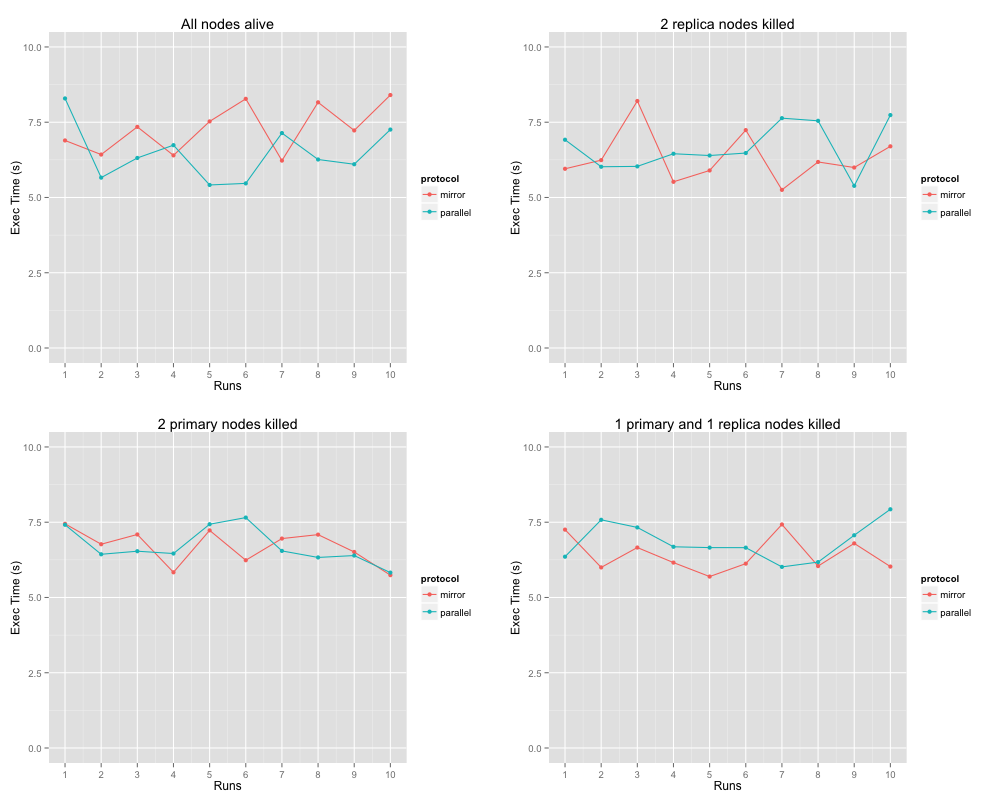
\includegraphics[width=16cm,height=12cm]{rb.png}
  \caption{Protocol performance comparison against red-black grid computing}
  \FloatBarrier
\end{figure}

Each sub-test ran for 10 times independently. The execution time is
measured in seconds. We see that for \emph{All nodes alive} scenario,
the parallel protocol performs slightly better than the mirror
protocol, this is because the overhead of synchronization between
senders and their replicas for parallel protocol is not as significant
as the overhead of sending/receiving redundant messages in mirror
protocol. In the other
three scenarios where two nodes were killed, they show similar
performance because as nodes were killed, parallel degrades to
mirror. 

\section*{My Test}
My test contains two loops. In the first loop, each node sends
messages to all other nodes and wait to receive the same message from
all other nodes. In the second loop, each node wait to receive
messages on MPI\_ANY\_SOURCE, while all other nodes send messages to
this node. All the messages are of the size of 8MB. The program first
ran the loops while all nodes were alive, then killed a primary node
and ran the loops again, then kill a replica node and ran the loops
for the last time. The result is shown in Figure 2.

\begin{figure}
  \centering
  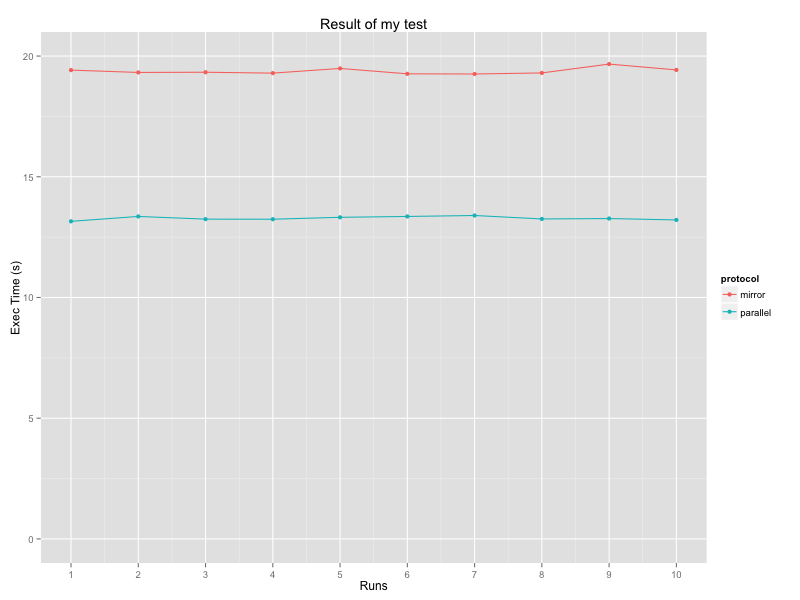
\includegraphics[width=10cm,height=8cm]{mytest.png}
  \caption{Protocol performance comparison against my test}
  \FloatBarrier
\end{figure}

We see that in this case, the parallel protocol shows a significant
performance advantage against the mirror protocol. It is because
the message size (8MB) here is relative large, thus the overhead of
redundant messages became the dominant factor in deciding the
performance.

\end{document}
